\documentclass[aspectratio=169,
				xcolor=table]{beamer}
\usepackage{ragged2e}
% Load general definitions
\usepackage[utf8]{inputenc}
%\usepackage[T1]{fontenc}
\usepackage[brazil]{babel}
\usepackage{amsmath}
\usepackage{amsfonts}
\usepackage{amssymb}
\usepackage{graphicx}
\usepackage{verbatim}
\usepackage{cancel}
\usepackage{askmaps}
\usepackage{tabularx}
\usepackage[table]{xcolor}
%\usepackage{tikz}
\usepackage{multirow}
\usepackage{mathtools}
\usepackage{color, colortbl}
\usepackage{etoolbox}
\usepackage{pbox}
\usepackage{changepage}
\usepackage{xpatch}
\usepackage{array}
\usepackage{marvosym}
\usepackage{tabu}
\usepackage{multicol}
\usepackage{listings}
\usepackage{underscore}
\usepackage{filecontents}
\usepackage[]{algorithm2e}
\usepackage{ragged2e}

\newcolumntype{P}[1]{>{\centering\arraybackslash}m{#1}}
\definecolor{Gray}{gray}{0.75}
\definecolor{Gray2}{gray}{0.85}

\definecolor{lightBlue}{HTML}{DAE8FC}
\definecolor{Blue}{RGB}{51, 51, 204}

%\useinnertheme[lily]{rounded}
\usetheme{UniEvangelica}
%\usetheme{Copenhagen}
%\usetheme{Berlin}
%\usecolortheme{dolphin}
\tolerance=1
\emergencystretch=\maxdimen
\hyphenpenalty=10000
\hbadness=10000

\setbeamertemplate{navigation symbols}{}%remove navigation symbols


\let\olditem=\item% 
\renewcommand{\item}{\olditem \justifying}%
\def\center{\trivlist \centering\item\relax}
\def\endcenter{\endtrivlist}

\setbeamertemplate{itemize/enumerate body begin}{\large}
\setbeamertemplate{itemize/enumerate subbody begin}{\large}

\setbeamertemplate{itemize item}{\raisebox{0.1ex}{$\blacktriangleright$}\hskip0.1em}
\setbeamertemplate{itemize subitem}{\raisebox{0.1ex}{$\blacktriangleright$}\hskip0.1em}

\newcommand{\greenarrow}{\textcolor{green}{\rotatebox[origin=c]{180}{\MVArrowDown}}}

\newcommand{\redarrow}{\textcolor{red}{\MVArrowDown}}

%\newcommand{\ftable}{
%	\begin{table}
%		\large
%		\centering
%		\rowcolors{1}{\ifnumless{\rownum}{2}{Blue}{lightBlue}}{}
%}

\newenvironment{eftable}{
	\begin{table}
		\large
		\centering
		\rowcolors{1}{}{Blue}
		\rowcolors{1}{\ifnumless{\rownum}{2}{Blue}{lightBlue}}{}
	}
	{
	\end{table}
}


%\setbeamertemplate{frametitle}
%{
%	%\vspace*{-2em}	
%	\insertframetitle
%
%	 %\textcolor{white}{\LARGE \insertframetitle}
%
%}

% Specific definitions
\title[]{Arquitetura e Organização de Computadores}
\subtitle[]{Unidade Central de Processamento - Parte 1}
\author[]{Prof. Alexandre Tannus}
\date{}

%\AtBeginSection{\frame{\sectionpage}}

\begin{document}

	\begin{frame}
		\titlepage
	\end{frame}

	\begin{frame}
		\tableofcontents		
	\end{frame}	
	
	\section{Introdução}
	\begin{frame}
		\frametitle{Unidade Central de Processamento (CPU)}
		\begin{itemize}
			\item \textit{Central Processing Unit} (CPU)
			\vspace{1em}
			\item Responsável pelos cálculos e controle da operação do computador

		\end{itemize}
		\begin{figure}
			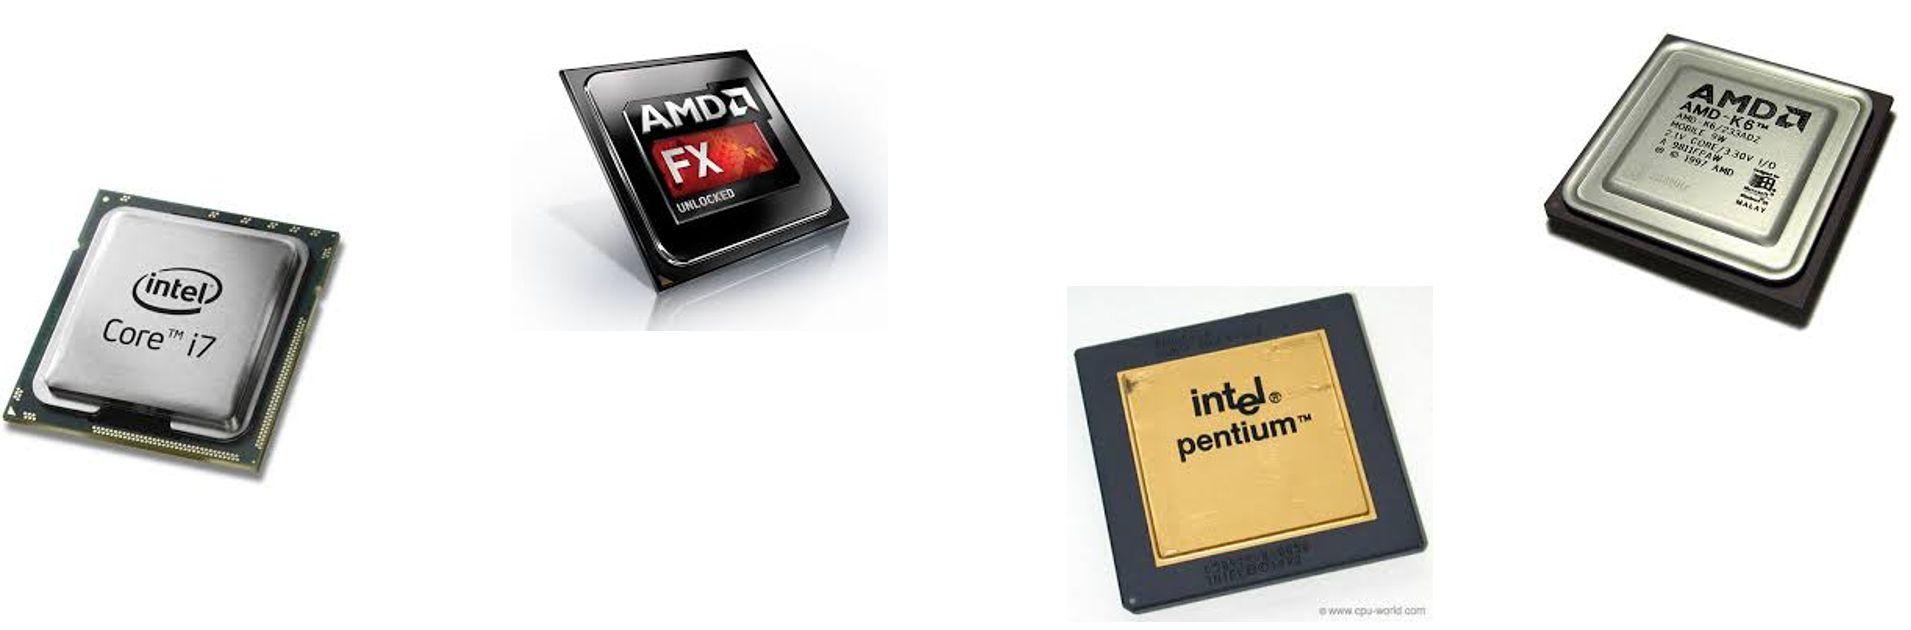
\includegraphics[height=3cm, keepaspectratio]{../figs/cap05/processadores.png} 
		\end{figure}
	\end{frame}
	
	\begin{frame}
		\frametitle{Estrutura da CPU}
		\begin{columns}
			\begin{column}{0.55\textwidth}
				\begin{itemize}
					\item Unidade lógica aritmética (ULA)
					\vspace{1em}
					\item Unidade de controle (UC)
					\vspace{1em}
					\item Registradores
					\vspace{1em}
					\item Barramentos

				\end{itemize}
			\end{column}
			\begin{column}{0.3\textwidth}
				\vspace{-0.5cm}
				\begin{figure}
					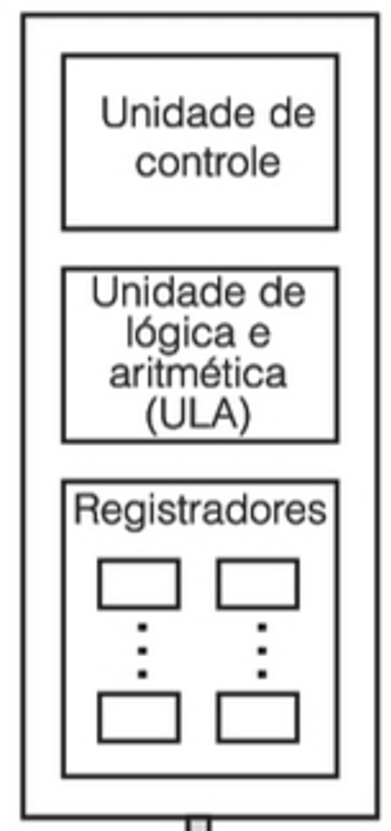
\includegraphics[height=5cm, keepaspectratio]{../figs/cap05/composicao.png} 
				\end{figure}				
			\end{column}
		\end{columns}
	\end{frame}
	
	\section{Unidade Lógica Aritmética}
		\begin{frame}
			\frametitle{CPU - Unidade Lógica Aritmética}
			\begin{itemize}
				\item Realiza as operações lógicas e aritméticas
				\begin{itemize}
					\item NOT, OR, AND
					\item Adição, Subtração
					\item Comparação
					\item Deslocamento
				\end{itemize}				
			\end{itemize}
			\begin{flushright}
				\begin{minipage}{0.7\textwidth}
					\vspace{-5em}
					\begin{figure}
						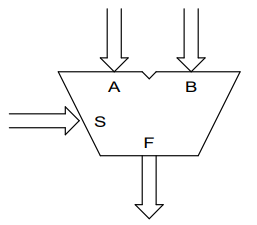
\includegraphics[height=0.6\textheight, keepaspectratio]{../figs/cap03/ula} 
					\end{figure}
				\end{minipage}
			\end{flushright}

		\end{frame}
		
		\begin{frame}
			\frametitle{Projeto da ULA - Representação de números}
				\begin{itemize}
					\item Inteiros sinalizados
					\begin{itemize}
						\item Sinal-magnitude
						\item \alert{Complemento de 2}
					\end{itemize}
					\vspace{1em}
					\item Ponto Flutuante
					\begin{itemize}
						\item \alert{Padrão ANSI/IEEE}
					\end{itemize}
				\end{itemize}
		\end{frame}		

		\begin{frame}
			\frametitle{Representação de inteiros: Sinal-magnitude}
			\begin{itemize}
				\item Bit mais significativo (MSB - \textit{Most Significant Bit}) indica o sinal
				\begin{itemize}
					\item 1: número negativo
					\item 0: número positivo
				\end{itemize}
			\end{itemize}
		\end{frame}		
	
		\begin{frame}
			\frametitle{Representação de inteiros: Complemento de 2}
			\begin{itemize}
				\item Representação de números negativos mais comum em hardware
	%			\pause
				\vspace{0.4em}
				\item Complemento de 1 $\to$ inversão bit a bit do número (complemento)
				\item Complemento de 2 $\to$ adição de 1 ao complemento de 1	
	%			\pause		
				\vspace{0.3em}
			\end{itemize}
			\begin{exampleblock}{Exemplos (representação em \textbf{8 bits})}
				\begin{columns}
					\begin{column}{0.45\textwidth}
						\begin{itemize}
							\item $9+4$
							\item $9-4$
						\end{itemize}
					\end{column}
					\begin{column}{0.45\textwidth}
						\begin{itemize}
							\item $-9+4$
							\item $-9-4$
						\end{itemize}
					\end{column}
				\end{columns}
			
			\end{exampleblock}
			
		\end{frame}		
		
		\begin{frame}
			\frametitle{Representação de ponto flutuante }
			\begin{eftable}
				\begin{tabular}{l | l | l}
					\textcolor{white}{Característica} &
					\textcolor{white}{Único/Curto} &
					\textcolor{white}{Duplo/Longo} \\
					Largura da palavra & 32 & 64 \\
					Bits mantissa & 23 & 52 \\
					Intervalo mantissa & $[1, 2-2^{-23}]$ & $[1, 2-2^{-52}]$\\
					Bits de expoente & 8 & 11 \\
					Excesso do expoente & 127 & 1023 \\
					Mínimo & $2^{-126} \approx 1,2x10^{-38}$ & $2^{-1022}\approx 2,2x10^{-308}$ \\
					Máximo & $2^{128} \approx 3,4x10^{-38}$ & $2^{1024}\approx 1,8x10^{308}$
				\end{tabular}
			
			\end{eftable}
		\end{frame}

		\begin{frame}
			\frametitle{Meio Somador - \textit{Half Adder}}
			\begin{columns}
				\begin{column}{0.3\textwidth}
					\begin{eftable}
						\begin{tabular}{c|c||c|c}		
							\textcolor{white}{x} & 
							\textcolor{white}{y} & 
							\textcolor{white}{s} & 
							\textcolor{white}{c} \\
							0 & 0 & 0 & 0 \\ 
							0 & 1 & 1 & 0 \\ 
							1 & 0 & 1 & 0 \\ 
							1 & 1 & 0 & 1 \\
						\end{tabular}		
					\end{eftable}				
				\end{column}
				\begin{column}{0.2\textwidth}
				\begin{figure}
					\hspace{-1cm}
					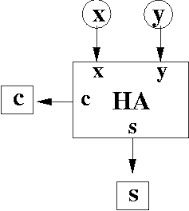
\includegraphics[height=3.4cm, keepaspectratio]{../figs/cap05/halfAdder.png} 
				\end{figure}
				\end{column}
				\begin{column}{0.5\textwidth}
					\begin{exampleblock}{Exemplos}
						\begin{itemize}
							\item $(11001)_2 + (1011)_2$ \\ 
		%					\pause
							\item $(101101)_2 + (11100111)_2$ \\ 
		%					\pause
							\item $(100111)_2 + (1110)_2 + (1011)_2 $			
						\end{itemize}
		
					\end{exampleblock}
				\end{column}
			\end{columns}
		\end{frame}

		\begin{frame}
			\frametitle{Somador Completo - \textit{Full Adder}}
			\begin{columns}
				\begin{column}{0.3\textwidth}
					\begin{eftable}
						\begin{tabular}{c|c|c||c|c}				
							\textcolor{white}{A} & 		
							\textcolor{white}{B} & 		
							\textcolor{white}{C-IN} & 		
							\textcolor{white}{C-OUT} & 		
							\textcolor{white}{SUM} \\ 
							0 & 0 & 0 & 0 & 0 \\ 
							0 & 0 & 1 & 0 & 1 \\ 
							0 & 1 & 0 & 0 & 1 \\ 
							0 & 1 & 1 & 1 & 0 \\ 
							1 & 0 & 0 & 0 & 1 \\ 
							1 & 0 & 1 & 1 & 0 \\ 
							1 & 1 & 0 & 1 & 0 \\ 
							1 & 1 & 1 & 1 & 1 \\ 
						\end{tabular} 
					\end{eftable}
				\end{column}
				\begin{column}{0.7\textwidth}
					\begin{figure}
						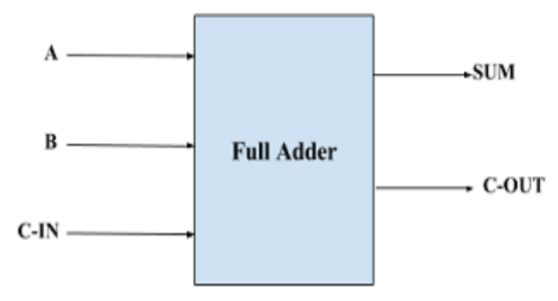
\includegraphics[width=.8\textwidth, keepaspectratio]{../figs/cap05/fullAdder.png} 
					\end{figure}
				\end{column}
			\end{columns}			
			
		\end{frame}


	\section{Barramentos}	
	
	\begin{frame}
		\frametitle{Barramentos}
		\begin{itemize}
			\item Vias que interligam os dispositivos (CPU, memória e periféricos), permitindo a comunicação entre os mesmos.
			\vspace{1em}
			\item Três tipos
			\begin{itemize}
				\item Dados
				\item Endereços
				\item Controle
			\end{itemize}
		\end{itemize}
		\begin{flushright}
		\begin{minipage}{0.7\textwidth}
			\vspace{-2.5cm}
			\begin{figure}
				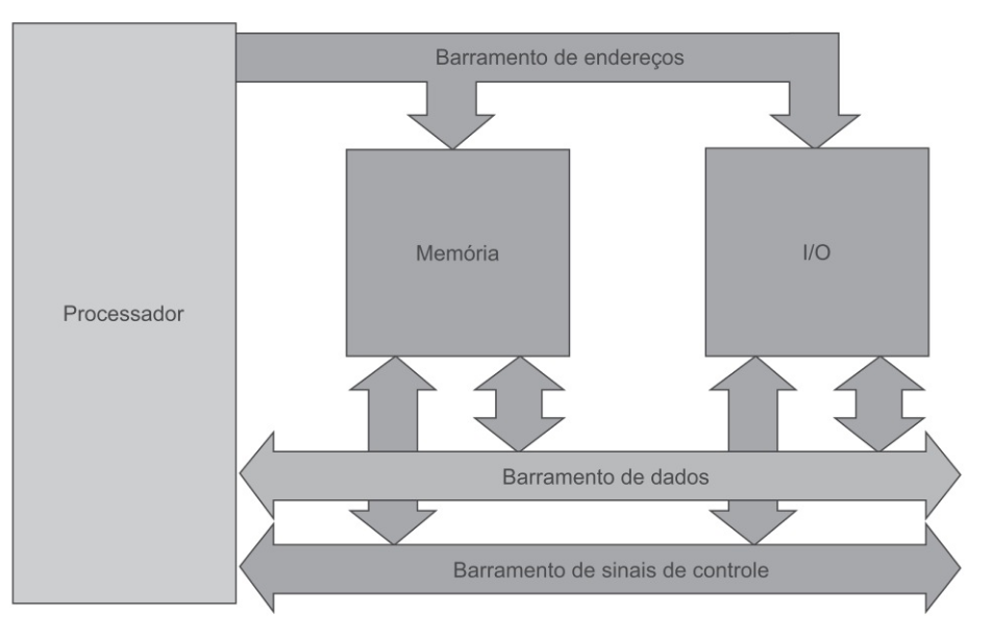
\includegraphics[width=.65\textwidth, keepaspectratio]{../figs/cap05/barramento.png}
			\end{figure}		
		\end{minipage}
		\end{flushright}
	\end{frame}
	
	\begin{frame}
		\frametitle{Barramento de dados}
		
		\begin{itemize}
			\item Trafega dados, informações ou instruções 
			\vspace{1em}
			\item Composto por vias
			\begin{itemize}
				\item Cada via trafega um bit
				\item Quantidade de vias define largura do barramento

			\end{itemize}
			\vspace{1em}
			
			\item \alert{ATENÇÃO: Largura do barramento de dados pode ser diferente da quantidade de bits que o processador utiliza} 			

		\end{itemize}
	\end{frame}
	
	\begin{frame}
		\frametitle{Barramento externo \textit{vs.} processamento interno}
		\begin{eftable}
			\begin{tabular}{l | c | c}
				\textcolor{white}{Processador} &
				\textcolor{white}{Processamento interno} &
				\textcolor{white}{Barramento externo} \\
				i8080 (1974) & 8 & 8 \\
				8088 (1979) & 16 & 8 \\
				80286 (1982) & 8 & 16 \\
				80386DX (1985) & 32 & 32 \\
				80486DX (1989) & 32 & 32 \\
				Pentium (1993) & 32 & 64 \\
				Athlon 64 (2003) & 64 & 128 			
			\end{tabular}
		\end{eftable}
	\end{frame}
	
	\begin{frame}
		\frametitle{Barramento de endereços}
		\begin{itemize}
			\item Endereçamento dos periféricos do sistema
			\begin{itemize}
				\item Memórias
				\item Controlador de vídeo
				\item Disco
				\item Rede

			\end{itemize}
			\vspace{1em}
			\item Quantidade de vias define quantidade máxima de endereços possíveis

		\end{itemize}
	\end{frame}
	
	\begin{frame}
		\frametitle{Barramento de endereço}
		\begin{eftable}
			\begin{tabular}{l | m{0.3\textwidth} | m{0.25\textwidth}}
				\textcolor{white}{Processador} & 
				\textcolor{white}{Largura do barramento  de endereços} & 
				\textcolor{white}{Quantidade máxima de endereços} \\
				i8088       & 20 bits & 1 Mb \\
				i80286      & 24 bits & 16 Mb \\
				i386        & 32 bits & 4 Gb  \\
				Pentium     & 32 bits & 4 Gb \\
				Core i5     & 35 bits & 32 Gb                         
			\end{tabular}
		\end{eftable}
	\end{frame}
	
	\begin{frame}
		\frametitle{Barramento de controle}
		\begin{itemize}
			\item Recebimento/envio de sinais de controle para os dispositivos do sistema
			\begin{itemize}
				\item RESET
				\item Interrupções
				\item HALT
				\item HOLD
				\item Seleção

			\end{itemize}
			\vspace{1em}
			\item Sinais de controle são específicos de cada arquitetura
		\end{itemize}
	\end{frame}
	
	\section{Registradores}
		\begin{frame}
			\frametitle{CPU - Registradores}
			\begin{itemize}
				\item Armazenam dados e instruções
				\vspace{1em}
				\item Baixa capacidade de armazenamento
				\vspace{1em}
				\item Alta velocidade de acesso
				\vspace{1em}
				\item Podem ser
				\begin{itemize}
					\item Propósito geral - operações lógicas e aritméticas
					\item Especiais - Acumuladores, \textit{Program Counter}, registrador de \textit{flags}, etc.
				\end{itemize}
				
			\end{itemize}
		\end{frame}
		
		\begin{frame}
			\frametitle{Registradores importantes}
			\begin{itemize}
				\item Contador de programa (\textit{Program Counter} - PC)	
				\begin{itemize}
					\item Armazena o endereço de memória onde será lida a próxima instrução que será executada
					\item Atualizado após a busca da instrução
				\end{itemize}
				\vspace{1em}
				\item Registrador de Instrução (\textit{Instruction Register} - IR)
				\begin{itemize}
					\item Armazena a instrução em execução
				\end{itemize}
			\end{itemize}
		\end{frame}
		
		\begin{frame}
			\frametitle{Registradores importantes}
			\begin{itemize}
			 \item Registrador de endereços de memória (\textit{Memory Address Registers} - MAR)
			 \vspace{1em}
			 \item Registrador \textit{buffer} de memória - (\textit{Memory Buffer Register} - MBR)
			\end{itemize}
			
			\vspace{1em}
			\Large \alert{Registradores responsáveis pela troca de informações (dados e instruções) entre memória e CPU}
		\end{frame}
		
		\begin{frame}
			\frametitle{Registradores importantes}
			\begin{itemize}
				\item Palavra de estado do programa ( \textit{Program State Word} - PSW)
				\vspace{1em}
				\item Informações de estado 
				\begin{itemize}
					\item sinal
					\item zero
					\item \textit{carry}: \textit{carry out} bit de uma operação
					\item \textit{overflow}
					\item  \textit{interrupt enable/disable}: habilita ou desabilita interrupções
				\end{itemize}
			\end{itemize}
		\end{frame}
		
		\begin{frame}
			\frametitle{Registradores de uso geral - Intel x86}
			\begin{itemize}
				\item AX - Acumuladores
				\item BX - Base
				\item CX - Contador
				\item DX - Dados
				\item BP - Ponteiro de base
				\item SI e DI - usado em operações que envolvem \textit{strings}
			\end{itemize}
			
		\end{frame}
	
	\section{Exercícios}	
	
	\begin{frame}
	
	Sobre Processadores, analise as assertivas e assinale a alternativa que aponta a(s) correta(s). 

I. A CPU é o 'cérebro' do computador, sua função é executar programas armazenados na memória principal, buscando suas instruções, examinando-as e então executando-as uma após a outra. 

\vspace{1em}
II. Barramentos podem ser externos à CPU, conectando-a à memória e aos dispositivos E/S, mas também podem ser internos à CPU. 

\vspace{1em}
III. A CPU é composta por várias partes distintas. A unidade de controle é responsável por buscar instruções na memória principal e determinar seu tipo. 

\vspace{1em}
IV. A unidade de aritmética e lógica efetua operações como adição AND (E) booleano para executar as intruções. 
	\end{frame}
	
	\begin{frame}
		Em relação à arquitetura, a CPU é representada pelo microprocessador, sendo responsável pela principal função dos microcomputadores, que é o processamento dos dados. Conceitualmente, a CPU é constituída de 
		
		\begin{enumerate}[a]
			\item Registradores / Memória Cache / Coprocessador Aritmético e Lógico.
			\item Registradores / Unidade de Controle / Unidade Lógica e Aritmética.
			\item Buffers / Memória Cache / Coprocessador Aritmético e Lógico.
			\item Buffers / Unidade de Controle / Unidade Lógica e Aritmética.
		\end{enumerate}


	\end{frame}
	
	
	\begin{frame}
	A CPU gera endereços que são colocados no barramento ...I.....e a memória os recebe através deste barramento. O caminho inverso desta operação não é possível (isso pode ser observado na figura). Durante a execução de um programa, cada instrução é levada até a ALU a partir da memória, uma instrução de cada vez, junto com qualquer dado que seja necessário para executá- la, cujo valor é transmitido através do barramento...II.... . A saída do programa é colocada em um dispositivo como um monitor de vídeo ou disco. A comunicação entre os componentes do sistema é sincronizada pelo barramento...III.. .

As lacunas I, II e III são correta e, respectivamente, preenchidas por:

	\begin{enumerate}[a]
		\normalsize
		\item De controle, de endereços,  de dados
		\item De endereços,  de dados, de sincronização
		\item De dados, de endereços, de controle
		\item De endereços,  de dados,  de controle
		\item Nenhuma das anteriores
	\end{enumerate}


	\end{frame}
	
	\begin{frame}
	Um computador com processador de 
	\begin{enumerate}[a]
		\normalsize
		\item 32 bits consegue endereçar um total de $2^{32}$ ou 8.294.967.295 endereços diferentes. Esses endereços apontam para a memória RAM, onde as informações de que o processador precisa ficam armazenadas. 
		\item 32 bits precisa ter, no mínimo, 4GB de RAM e velocidade de clock mínima de 3.2GHz. Estes dados garantem que o sistema operacional possa ser carregado na BIOS sem problemas. 
		\item 64 bits precisa ter, no mínimo, 8GB de RAM e velocidade de clock mínima de 6.4GHz. Estes dados garantem que o sistema operacional possa ser carregado na ROM sem problemas
		\item 64 bits consegue endereçar $2^{64}$ endereços diferentes, podendo acessar muito mais RAM. Mas computadores pessoais atuais raramente suportam mais que 64GB de RAM. 
		\item 32 bits ou de 64 bits consegue acessar 8GB de RAM, mas o de 64 bits consegue acessá-la de maneira mais rápida e eficiente, o que deixa o computador mais rápido também. 
	\end{enumerate}

	\end{frame}
	
	\begin{frame}
		\frametitle{Verdadeiro ou Falso}
		A função do registro de instrução é armazenar o identificador da próxima instrução a ser executada pelo processador.
	\end{frame}
	
	\begin{frame}
		\frametitle{Verdadeiro ou Falso}
		Se, para reduzir custos de fabricação, for criado um computador em que o tamanho do registrador PC (program counter) seja a metade do REM, então, embora ocorra a redução do custo, essa máquina não irá funcionar, pois o PC deve ser projetado, no mínimo, com o mesmo tamanho do REM.
	\end{frame}
	
\end{document}